\documentclass{elektr}
\usepackage[all]{xy}
\usepackage{amsfonts,amssymb,amsmath,amsgen,amsopn,amsbsy,theorem,graphicx,epsfig}
\usepackage{amscd,bezier,latexsym,mathrsfs,eurosym,enumerate}
\usepackage[utf8]{inputenc}
\usepackage[english]{babel}
\usepackage{multirow}
\usepackage[dvipsnames]{xcolor}
\usepackage[pagewise]{lineno}
\usepackage{booktabs,tabularx,float,placeins}
\usepackage{algorithm}
\usepackage{algpseudocode}
\usepackage{tikz}
\usetikzlibrary{arrows.meta,positioning}
\definecolor{teal}{RGB}{0,128,128}
\definecolor{gold}{RGB}{218,165,32}
\definecolor{navy}{RGB}{0,0,128}
\newcolumntype{L}[1]{>{\raggedright\arraybackslash}p{#1}}
\newcolumntype{Y}{>{\raggedright\arraybackslash}X}
\tikzset{
box/.style={draw,rounded corners,align=center,fill=blue!5,inner sep=5pt},
arrow/.style={-{Latex[length=2mm]},thick}
}
\newcommand{\safeincludegraphics}[2][]{%
  \IfFileExists{#2}{\includegraphics[#1]{#2}}{%
    \fbox{\parbox[c][32mm][c]{0.82\linewidth}{\centering
      External figure not supplied:\\[0.4ex]\texttt{\detokenize{#2}}}}}}
\usepackage{hyperref}
\hypersetup{
colorlinks=true,
urlcolor=black,
citecolor=blue}
\usepackage{cleveref}
\makeatletter
\renewcommand{\theHALG@line}{\thealgorithm.\arabic{ALG@line}}
\makeatother
\linenumbers

\yil{}
\vol{}
\fpage{}
\lpage{}
\doi{}

\title{An Explainable Logistic-Meta-Learner Stacking Framework with Domain-Informed Feature Engineering for Multiclass Sleep-Disorder Risk Stratification}

\author[AUTHOR and AUTHOR]{
	\textbf{Rifat Bin Reza$^{1,}$\thanks{rifat.bin.reza1@g.bracu.ac.bd}~, Md Ahadul Haque Suvo$^{2}$, Atair Rahman Alvi$^{1}$}\\
	$^{1}$BSRM School of Engineering, Department of Electrical and Electronics Engineering, Brac University, Dhaka, Bangladesh\\ 	
	$^{2}$Aviation and Aerospace University, Department of Avionics Engineering, Dhaka, Bangladesh\\
  First AUTHOR: \url{https://orcid.org/0009-0006-1865-8419} \\
  Second AUTHOR: \url{https://orcid.org/0009-0000-6756-4773} \\
  Third AUTHOR: \url{https://orcid.org/0009-0006-5117-8599} \\
  \\ 
\rec{...}
\acc{...}
\finv{...}
}

\def\E{\ifmmode{\mathbb E}\else{$\mathbb E$}\fi} %natural numbers
\def\N{\ifmmode{\mathbb N}\else{$\mathbb N$}\fi} %natural numbers
\def\R{\ifmmode{\mathbb R}\else{$\mathbb R$}\fi} %real numbers
\def\Q{\ifmmode{\mathbb Q}\else{$\mathbb Q$}\fi} %rational numbers
\def\C{\ifmmode{\mathbb C}\else{$\mathbb C$}\fi} %complex numbers
\def\H{\ifmmode{\mathbb H}\else{$\mathbb H$}\fi} %complex numbers
\def\Z{\ifmmode{\mathbb Z}\else{$\mathbb Z$}\fi} %integers
\def\P{\ifmmode{\mathbb P}\else{$\mathbb P$}\fi} %real numbers
\def\T{\ifmmode{\mathbb T}\else{$\mathbb T$}\fi} %real numbers
\def\SS{\ifmmode{\mathbb S}\else{$\mathbb S$}\fi} %real numbers
\def\DD{\ifmmode{\mathbb D}\else{$\mathbb D$}\fi} %real numbers

\renewcommand{\a}{\alpha}
\renewcommand{\b}{\beta}
\renewcommand{\d}{\delta}
\newcommand{\D}{\Delta}
\newcommand{\e}{\epsilon}
\newcommand{\var}{\varepsilon}
\newcommand{\g}{\gamma}
\newcommand{\la}{\lambda}
\newcommand{\La}{\Lambda}
\newcommand{\lan}{\langle}
\newcommand{\ran}{\rangle}
\newcommand{\n}{\nabla}
\newcommand{\va}{\varphi}
\newcommand{\s}{\sigma}
\newcommand{\Sig}{\Sigma}
\renewcommand{\t}{\tau}
\renewcommand{\th}{\theta}
\newcommand{\Om}{\Omega}
\newcommand{\om}{\omega}
\newcommand{\pa}{\partial}
\newcommand{\up}{\upsilon}
\newcommand{\vp}{\varphi}
\newcommand{\z}{\zeta}





\newcommand{\bse}{\begin{subequations}}
\newcommand{\ese}{\end{subequations}}
\newcommand{\ben}{\begin{enumerate}}
\newcommand{\een}{\end{enumerate}}
\newcommand{\bens}{\begin{enumerate*}}
\newcommand{\eens}{\end{enumerate*}}
\newcommand{\be}{\begin{equation}}
\newcommand{\ee}{\end{equation}}
\newcommand{\bea}{\begin{eqnarray}}
\newcommand{\eea}{\end{eqnarray}}
\newcommand{\baa}{\begin{eqnarray*}}
\newcommand{\eaa}{\end{eqnarray*}}
\newcommand{\bc}{\begin{center}}
\newcommand{\ec}{\end{center}}
\newcommand{\ol}{\overline}
\newcommand{\ul}{\underline}
\newcommand{\ov}{\overbrace}
\newcommand{\uv}{\underbrace}
\newcommand{\Ra}{\Rightarrow}
\newcommand{\ra}{\rightarrow}
\newcommand{\ds}{\displaystyle}
\newcommand{\vs}{\vspace}


\newcommand{\IR}{\mbox{I \hspace{-0.2cm}R}}
\newcommand{\IN}{\mbox{I \hspace{-0.2cm}N}}



%% \theoremstyle{plain} %% This is the default

\newtheorem{theorem}{Theorem}%[section]

\newtheorem{corollary}{Corollary}

\newtheorem{lemma}{Lemma}

\newtheorem{proposition}{Proposition}

\newtheorem{axiom}{Axiom}

\newtheorem{conjecture}{Conjecture}

\newtheorem{example}{Example}

\newtheorem{definition}{Definition}%[section]

\newtheorem{remark}{Remark}%[section]
\newtheorem{notation}{Notation}


\newtheorem{question}{Question}%[section]
\newtheorem{construction}{Construction}

\newtheorem{athm}{Theorem}
\renewcommand{\theathm}{\Alph{athm}}




\setcounter{page}{1}
\begin{document}
\raggedbottom
% Compact journal layout: keep floats/equations close to the discussion.
\setlength{\textfloatsep}{7pt plus 2pt minus 2pt}
\setlength{\floatsep}{6pt plus 2pt minus 2pt}
\setlength{\intextsep}{6pt plus 2pt minus 2pt}
\setlength{\abovedisplayskip}{5pt plus 2pt minus 2pt}
\setlength{\belowdisplayskip}{5pt plus 2pt minus 2pt}
\setlength{\abovedisplayshortskip}{3pt plus 1pt minus 1pt}
\setlength{\belowdisplayshortskip}{3pt plus 1pt minus 1pt}
\renewcommand{\arraystretch}{0.93}

\maketitle

\begin{abstract}Accurate risk stratification may facilitate timely referral for sleep assessment, yet models developed from small tabular datasets are particularly susceptible to outcome ambiguity, preprocessing leakage, and optimistic validation. This study develops an explainable stacking framework using the publicly available Sleep Health and Lifestyle Dataset, comprising 374 participant-level observations, 11 mixed-type predictors, and three outcome categories: no recorded disorder, insomnia, and sleep apnea. Administrative identifiers were excluded, blood pressure was decomposed into systolic and diastolic components, and every data-dependent transformation was estimated exclusively from the training partition. Random Forest, XGBoost, and a radial-basis-function support vector machine were integrated as base learners through a logistic-regression meta-learner fitted to out-of-fold class probabilities and the encoded predictor pass-through. Model behaviour was examined using complementary SHAP and LIME analyses, a class-separability diagnostic based on principal component analysis, and a two-dimensional Accumulated Local Effects surface, while discrimination was assessed on a stratified 20\% hold-out set and summarised with one-vs-rest ROC--AUC. The proposed stack correctly classified 73 of 75 observations, corresponding to an accuracy of 97.33\% and a macro-F1 score of 0.96, with a macro-average ROC--AUC of 0.997. Class-specific F1 scores were 0.93 for insomnia, 1.00 for no recorded disorder, and 0.94 for sleep apnea. The RF--XGBoost soft-voting comparator achieved 96.00\% accuracy on the same partition. A repeated-split robustness check across 13 additional stratified partitions indicated a mean test accuracy of 0.924 (SD 0.027) for the proposed stack, consistent with the single-split result. These findings establish a reproducible computational benchmark rather than a clinically deployable diagnostic system. Independent outcome adjudication, repeated internal validation, calibration analysis, and prospective external evaluation remain necessary.

\keywords{Sleep disorder, insomnia, sleep apnea, stacking ensemble, XGBoost, explainable machine learning, clinical decision support}
\end{abstract}

\section{Introduction}
Sleep disorders comprise clinically heterogeneous conditions with distinct diagnostic criteria and management pathways. The 2023 text revision of the International Classification of Sleep Disorders separates insomnia disorders from sleep-related breathing disorders, whereas the benchmark used here compresses this richer taxonomy into three coarse outcome categories \cite{aasm2023}. Obstructive sleep apnea is especially relevant to screening research because conventional diagnostic pathways remain resource intensive and access to definitive testing is uneven \cite{korkalainen2024,giorgi2025,bazoukis2023}. A data-driven model may therefore assist referral prioritisation, but it cannot establish a diagnosis from lifestyle attributes alone.

Structured lifestyle and physiological data offer a pragmatic basis for methodological development, but they also create substantial analytical risk. Predictors differ in scale and representation, categorical levels require harmonisation, and the outcome classes are unequal. Performance can be materially inflated when preprocessing precedes data partitioning, model choices are adapted to evaluation results, or uncertainty from a small test sample is ignored \cite{kapoor2023,efthimiou2024,collins2024}. Reliable evaluation consequently requires strict separation of development and test data, class-sensitive metrics, paired uncertainty analysis, and explicit limits on transportability and clinical interpretation.

This study addresses these requirements through five contributions. First, it specifies an auditable preprocessing strategy for mixed numerical and categorical variables, with all learned transformations confined to the development partition. Second, it develops a heterogeneous stack \cite{wolpert1992} in which Random Forest \cite{breiman2001}, XGBoost \cite{chen2016}, and a radial-basis-function support vector machine \cite{cortes1995} contribute out-of-fold class probabilities and the encoded predictors are passed to a logistic meta-learner. Third, it evaluates the proposed model against soft voting and previously reported ANN ensembles, including a repeated-split robustness check. Fourth, it combines SHAP \cite{lundberg2017}, LIME \cite{ribeiro2016}, a PCA-based class-separability diagnostic, and a two-dimensional Accumulated Local Effects surface \cite{apley2020} to examine global importance, local attribution, and feature-interaction patterns while explicitly separating predictive association from causal or diagnostic interpretation \cite{jung2023,allen2024,pesapane2026}. Fifth, it reports one-vs-rest ROC--AUC \cite{fawcett2006} alongside threshold-based metrics to characterise ranking quality independently of the classification threshold.

\section{Related work and study rationale}
Recent sleep-AI research has concentrated primarily on apnea detection from physiological signals and wearable devices. Contemporary reviews cover electrocardiographic, oximetric, respiratory, and multimodal signal pipelines, and consistently distinguish automated screening from clinically adjudicated diagnosis \cite{bazoukis2023,tyagi2023,abdalrazaq2024,giorgi2025}. This evidence base is informative for clinical framing but is not directly comparable with the present low-dimensional lifestyle dataset, which contains neither raw physiological waveforms nor polysomnographic severity indices.

For tabular prediction, recent evidence continues to treat tree ensembles and neural architectures as complementary rather than universally interchangeable model families \cite{borisov2024}. Alom et al. applied ANN bagging, boosting, and weighted averaging to the same sleep-health benchmark used here \cite{alom2024}; their reported accuracies provide the only literature-derived numerical comparator in this manuscript. In a different clinical setting, Alabi et al. demonstrated that heterogeneous stacking can be paired with SHAP and LIME on a cancer-survival task, supporting the general strategy of combining stacking with SHAP/LIME explanation, although their sample construction and validation design preclude direct performance comparison \cite{alabi2023}. Bazoukis et al. and Tyagi et al. review machine-learning and deep-learning pipelines applied to physiological sleep signals, providing clinical screening context rather than a tabular-benchmark comparator \cite{bazoukis2023,tyagi2023}. Borisov et al. survey tree-based and neural architectures on tabular data generally, supporting the use of heterogeneous, non-neural base learners such as the RF--XGBoost--SVM combination adopted here \cite{borisov2024}. The unresolved methodological question is therefore whether an out-of-fold RF--XGBoost--SVM stack can improve discrimination on this specific benchmark while maintaining strict evaluation separation and transparent uncertainty.

The explanation layer is deliberately bounded. Recent reviews emphasise that post-hoc explanations require explicit definitions of audience, fidelity, stability, and intended use; an attribution is evidence about a fitted prediction function, not a causal mechanism or clinical rationale \cite{jung2023,allen2024}. Likewise, current reporting and deployment guidance requires transparent data provenance, evaluation design, uncertainty, and validation before clinical use \cite{tripodai2024,futureai2025}. Accordingly, all ANN percentages in the comparative results are transcribed from Alom et al. \cite{alom2024}, whereas every RF--XGBoost--SVM value is generated by the present analysis. The comparison is descriptive because the studies do not share an identical evaluation protocol.

\section{Materials and Methods}

\subsection{Methodological overview}
The investigation followed a leakage-controlled analytical pathway (Figure~\ref{fig:workflow}). Data integrity and outcome coding were examined before modelling, after which the administrative identifier was removed and clinically interpretable features were derived. A stratified test partition was then isolated prior to fitting any transformation. Within the development partition, numerical variables were standardised, categorical variables were one-hot encoded, and out-of-fold probability estimates were generated for all three base learners. These estimates and the encoded predictors formed the input to a logistic-regression meta-learner through the implemented pass-through connection. Final discrimination, paired model comparisons, and explanation analyses were conducted only after the complete pipeline had been fixed. This design preserves the independence of the test set and prevents information from the evaluation sample from influencing representation learning or model construction.

\begin{figure}[H]
\centering
\safeincludegraphics[width=\linewidth]{../1.png}
\caption{End-to-end framework for leakage-controlled, explainable RF--XGBoost--SVM stacking. Stages 1--2 correspond to data definition and leakage-controlled preprocessing; Stage 3 is the stratified development--test partition; Stage 4 is the out-of-fold RF--XGBoost--SVM stacking architecture; and Stage 5 covers hold-out evaluation and post-hoc explanation.}
\label{fig:workflow}
\end{figure}

\subsection{Problem formulation and notation}
Let the benchmark sample be $\mathcal{D}=\{(\mathbf{x}_i,y_i)\}_{i=1}^{N}$, where $N=374$, $\mathbf{x}_i\in\mathbb{R}^{d_n}\times\mathcal{A}^{d_c}$ contains numerical and categorical predictors, and $y_i\in\mathcal{C}=\{0,1,2\}$ denotes insomnia, no recorded disorder, or sleep apnea. The analytical objective is to estimate a probabilistic mapping
\begin{equation}
F:\mathcal{X}\rightarrow\Delta^{C-1},\qquad
\hat y_i=\arg\max_{c\in\mathcal{C}}F_c(\mathbf{x}_i),
\label{eq:problem}
\end{equation}
where $C=3$ and $\Delta^{C-1}$ is the probability simplex. The stratified partition satisfies
\begin{equation}
\mathcal{D}_{tr}\cap\mathcal{D}_{te}=\varnothing,
\qquad |\mathcal{D}_{tr}|=299,
\qquad |\mathcal{D}_{te}|=75,
\label{eq:partition}
\end{equation}
and every estimated parameter is a function of $\mathcal{D}_{tr}$ only. For numerical predictor $j$, development-set standardisation is
\begin{equation}
\widetilde{x}_{ij}=\frac{x_{ij}-\mu^{(tr)}_j}{\sigma^{(tr)}_j},
\quad
\mu^{(tr)}_j=\frac{1}{n_{tr}}\sum_{i\in\mathcal{D}_{tr}}x_{ij},
\label{eq:standardise}
\end{equation}
where $\sigma^{(tr)}_j$ is the sample standard deviation estimated from $\mathcal{D}_{tr}$. A categorical level $a_q$ is represented by $o_{iq}=\mathbb{I}(x_{ij}=a_q)$. Consequently, the fitted transformer $T_{\widehat{\theta}_{tr}}$ maps each observation to the fixed-schema vector $\mathbf{x}'_i=T_{\widehat{\theta}_{tr}}(\mathbf{x}_i)$, with neither the scale parameters nor the categorical vocabulary re-estimated on the test partition.

\subsection{Data source and outcome definition}
The analysis used the publicly available Sleep Health and Lifestyle Dataset hosted on Kaggle \cite{kaggle2023}. The dataset comprises 374 participant-level observations and 13 variables: one administrative identifier (Person ID), 11 candidate predictors, and the Sleep Disorder outcome. The predictors span demographic characteristics (age, gender, occupation), sleep behaviour (sleep duration, quality of sleep), lifestyle indicators (physical activity level, daily steps), psychophysiological measures (stress level, heart rate), anthropometric category (BMI category), and cardiovascular status (blood pressure, later split into systolic and diastolic values). Because the data were not collected as a prospectively recruited clinical cohort and the outcome was not independently adjudicated, the dataset is treated as a methodological benchmark for risk stratification rather than as a source of prevalence estimates or diagnostic ground truth.

All 11 predictors were complete, whereas 219 of 374 outcome entries were blank. Consistent with the coding used in the analytical dataset, blank outcomes were assigned to the no-recorded-disorder category, producing 219 observations with no recorded disorder, 77 with insomnia, and 78 with sleep apnea. This operational definition is consequential because absence of a recorded label is not equivalent to clinician-confirmed absence of disease. The assignment was therefore retained for reproducibility but treated as a primary source of outcome uncertainty throughout interpretation.

Age ranged from 27 to 59 years (mean 42.18, standard deviation 8.67), and reported sleep duration ranged from 5.8 to 8.5 h (mean 7.13, standard deviation 0.80). Quality-of-sleep scores ranged from 4 to 9, physical-activity levels from 30 to 90, stress scores from 3 to 8, heart rate from 65 to 86 beats/min, and daily step counts from 3,000 to 10,000. The categorical variables comprised two gender categories, 11 occupational groups, and four body-mass-index labels. Blood pressure, originally represented as a systolic/diastolic string, was separated into two numerical variables. The synonymous labels ``Normal Weight'' and ``Normal'' were consolidated before one-hot encoding. Person ID was excluded because it contains ordering information without a plausible physiological interpretation. Occupation was retained as a contextual predictor, although its contribution requires careful scrutiny because it may encode socioeconomic structure and introduce transportability concerns. The public-source provenance, modest sample size, outcome-assignment rule, and absence of clinical adjudication therefore define the inferential boundaries of this study.

\subsection{Class separability diagnostic (PCA) and feature relationships}
\label{sec:pca}
To characterise the intrinsic separability of the three outcome classes independent of any specific classifier, a two-component principal component analysis was fitted to the fully preprocessed (scaled and one-hot encoded) feature matrix using all 374 observations. This projection is diagnostic only: it is fitted separately from, and never substituted into, the classification pipeline described in Sections~3.6--3.7, so it does not affect any reported classification metric. The first two components explained 33.68\% and 29.47\% of total variance respectively (63.14\% combined), indicating that a large share of the feature-space structure is not captured in two dimensions and that any apparent overlap in the projection understates the information available to the full-dimensional classifiers.

Two further diagnostics were used to examine dependence structure among predictors and the fitted stack's local behaviour: Spearman rank correlation across the nine numerical predictors on the development partition, and a two-dimensional Accumulated Local Effects (ALE) surface computed directly from the fitted stacking pipeline for the joint effect of Sleep Duration and Quality of Sleep on the predicted probability of insomnia, using a $6\times6$ quantile grid. Unlike SHAP, ALE conditions on the local data density and is therefore less sensitive to feature correlation when estimating joint effects; it was accumulated by summing corner-difference finite effects across grid cells and centring the resulting surface to zero mean.

Figure~\ref{fig:datapca}a shows the raw PCA scatter, and Figure~\ref{fig:datapca}b overlays 1-sigma covariance ellipses per class. The no-recorded-disorder class occupies a visually distinct region, consistent with its perfect recall in Table~\ref{tab:metrics}, whereas the insomnia and sleep-apnea ellipses show partial overlap. This is consistent with, though not a direct explanation for, the two insomnia-to-apnea misclassifications reported in Section~5. Figure~\ref{fig:datapca}c shows that Sleep Duration and Quality of Sleep are strongly positively correlated, while Stress Level is negatively correlated with both, consistent with their combined appearance among the higher-ranked SHAP features in Section~5.3. Figure~\ref{fig:datapca}d shows the corresponding ALE surface: the predicted insomnia probability rises most sharply in the region of short sleep duration combined with low sleep quality, and flattens once both variables exceed their sample medians, indicating a joint rather than additive relationship between these two predictors and the insomnia class score. As with SHAP and LIME, the PCA and ALE diagnostics characterise structure and the fitted function's local behaviour respectively, and neither should be read as a causal relationship.

\begin{figure}[H]
\centering
\begin{minipage}[t]{0.48\linewidth}
\centering\textbf{(a)--(b)}\\[0.3ex]
\safeincludegraphics[width=\linewidth]{pca_class_separability.png}
\end{minipage}\hfill
\begin{minipage}[t]{0.48\linewidth}
\centering\textbf{(c)--(d)}\\[0.3ex]
\safeincludegraphics[width=\linewidth]{feature_relationships_ale.png}
\end{minipage}
\caption{Data-structure diagnostics (not part of the modelling pipeline): (a) PCA scatter by outcome class and (b) the same projection with 1-sigma class ellipses (PC1 = 33.68\% variance, PC2 = 29.47\% variance); (c) Spearman rank correlation among numerical predictors on the development partition; (d) two-dimensional Accumulated Local Effects surface for Sleep Duration and Quality of Sleep on the stacking classifier's predicted probability of insomnia.}
\label{fig:datapca}
\end{figure}

\FloatBarrier

\subsection{Data splitting and leakage control}
An 80:20 stratified partition with random seed 42 produced a development set of 299 observations and an independent test set of 75 observations. The split was performed before numerical scaling, categorical encoding, or model fitting. All preprocessing parameters, including numerical means and variances, categorical vocabularies, and label mappings, were estimated from the development data and subsequently applied without modification to the test set. The same principle was maintained within cross-validation folds used to construct the stack. This ordering prevents evaluation-set information from influencing either the feature representation or the fitted decision function \cite{kapoor2023,efthimiou2024}.

\paragraph{Leakage-controlled preprocessing.}
After removing Person ID, blank outcomes were mapped to the operational ``no recorded disorder'' class, BMI labels were harmonised, and blood pressure was split into systolic and diastolic values. An 80:20 stratified split (seed 42) was then created. Numerical standardisation, categorical one-hot encoding, and label mapping were fitted on the development partition only and applied unchanged to the test partition. The same fold-local fitting rule was used while generating out-of-fold predictions for stacking.

\subsection{Base Learners and Stacking Design}
The heterogeneous stack used Random Forest (RF), XGBoost, and a radial-basis-function support vector machine (RBF-SVM). RF used 100 trees, maximum depth 10, minimum split size 5, minimum leaf size 1, and seed 42. XGBoost used 800 estimators, learning rate 0.02, maximum depth 3, row/column subsampling 0.90, minimum child weight 3, $\gamma=0.15$, and $\lambda=1.2$. The RBF-SVM supplied calibrated class-probability estimates; the available experiment record does not specify non-default SVM hyperparameters, so no additional values are asserted here.

For each development observation, five-fold stratified cross-validation generated class-probability vectors from models that excluded that observation. If $\kappa(i)$ is the fold containing observation $i$, the meta-level vector is
\begin{equation}
\mathbf{z}^{OOF}_i=\left[{\mathbf{x}'_i}^{\!\top},
{\mathbf{p}_{RF}^{(-\kappa(i))}}^{\!\top},
{\mathbf{p}_{XGB}^{(-\kappa(i))}}^{\!\top},
{\mathbf{p}_{SVM}^{(-\kappa(i))}}^{\!\top}\right]^{\!\top}\in\mathbb{R}^{d+3C}.
\label{eq:oofvector}
\end{equation}
A multinomial logistic-regression meta-learner with encoded-feature pass-through and $C_{\mathrm{LR}}=2.0$ then estimated
\begin{equation}
p_{S}(c\mid\mathbf{z})=
\frac{\exp(\beta_{c0}+\boldsymbol{\beta}_c^{\top}\mathbf{z})}
{\sum_{r=1}^{C}\exp(\beta_{r0}+\boldsymbol{\beta}_r^{\top}\mathbf{z})}.
\label{eq:meta}
\end{equation}
After meta-learner fitting, all three base learners were refitted on the complete development set. For test observation $x'$, the final meta-vector was $z^*=[x',p_{RF},p_{XGB},p_{SVM}]$, and the predicted class was $\hat y=\arg\max_c p_S(c\mid z^*)$. Restricting meta-training to out-of-fold probabilities prevents second-level exposure to optimistically biased in-sample predictions \cite{kapoor2023,alabi2023}.

\begin{table}[H]
\centering
\caption{Model and validation configuration used in the proposed stack.}
\label{tab:hyper}
\scriptsize
\begin{tabular}{lll}
\toprule
Component & Parameter & Value \\
\midrule
Random Forest & trees / max depth / min split & 100 / 10 / 5 \\
XGBoost & estimators / learning rate / max depth & 800 / 0.02 / 3 \\
 & row / column subsample & 0.90 / 0.90 \\
 & min child weight / $\gamma$ / $\lambda$ & 3 / 0.15 / 1.2 \\
RBF-SVM & kernel / output & RBF / class probabilities \\
Meta-learner & model / $C_{\mathrm{LR}}$ / solver & logistic / 2.0 / L-BFGS \\
 & encoded-feature pass-through & enabled \\
Validation & split / seed / stacking folds & 80:20 stratified / 42 / 5 \\
\bottomrule
\end{tabular}
\end{table}

\begin{figure}[H]
\centering
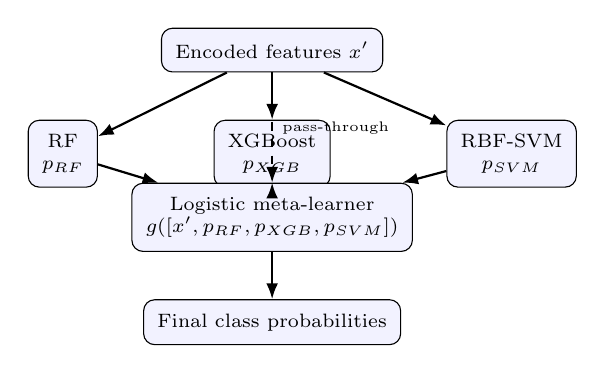
\begin{tikzpicture}[node distance=6mm and 8mm, every node/.style={font=\scriptsize}]
\node[box] (x) {Encoded features $x'$};
\node[box,below left=of x] (rf) {RF\\$p_{RF}$};
\node[box,below=of x] (xgb) {XGBoost\\$p_{XGB}$};
\node[box,below right=of x] (svm) {RBF-SVM\\$p_{SVM}$};
\node[box,below=14mm of x] (meta) {Logistic meta-learner\\$g([x',p_{RF},p_{XGB},p_{SVM}])$};
\node[box,below=of meta] (y) {Final class probabilities};
\draw[arrow] (x)--(rf); \draw[arrow] (x)--(xgb); \draw[arrow] (x)--(svm);
\draw[arrow] (rf)--(meta); \draw[arrow] (xgb)--(meta); \draw[arrow] (svm)--(meta);
\draw[arrow,dashed] (x)--node[right,font=\tiny]{pass-through} (meta); \draw[arrow] (meta)--(y);
\end{tikzpicture}
\caption{Proposed RF--XGBoost--SVM stack. Out-of-fold class probabilities from all three base learners are concatenated with the encoded predictor pass-through and supplied to the logistic meta-learner.}
\label{fig:stack}
\end{figure}

\subsection{Explainability and Auditability}
SHAP explanations were obtained through a permutation-based, model-agnostic interface. A fixed background sample $B$ was drawn exclusively from the development partition, and each perturbed observation was passed through the complete preprocessing and prediction pipeline. For class $c$, local additive consistency satisfies
\begin{equation}
F_c(\mathbf{x}_i)-\mathbb{E}_{\mathbf{X}\sim B}[F_c(\mathbf{X})]
=\sum_{j=1}^{d}\phi_{ij}^{(c)},
\label{eq:shaplocal}
\end{equation}
and global importance for feature $j$ was defined as
\begin{equation}
I_j=\frac{1}{nC}\sum_{i=1}^{n}\sum_{c=1}^{C}|\phi_{ij}^{(c)}|.
\label{eq:shapglobal}
\end{equation}
Here, $\phi_{ij}^{(c)}$ denotes the attribution assigned to feature $j$ for observation $i$ and class $c$. LIME was used as a complementary local analysis. Given perturbed neighbourhood $\mathcal{Z}_i$, proximity kernel $\pi_i$, and interpretable surrogate family $\mathcal{G}$, the local explanation is
\begin{equation}
g_i^{*}=\arg\min_{g\in\mathcal{G}}
\left\{\sum_{\mathbf{z}\in\mathcal{Z}_i}\pi_i(\mathbf{z})
[F_c(\mathbf{z})-g(\mathbf{z})]^2+\Omega(g)\right\},
\label{eq:lime}
\end{equation}
where $\Omega(g)$ penalises surrogate complexity. Absolute LIME coefficients were aggregated only to assess broad agreement with SHAP rankings; they were not treated as a second estimate of causal importance. Both methods characterise the fitted prediction function, and their outputs depend on the chosen background distribution, perturbation mechanism, and representation of predictor dependence \cite{instanceshap2023,jung2023}.

\FloatBarrier
\section{Experimental protocol}
The evaluation used the isolated 75-observation test partition. Accuracy was reported alongside class-specific precision, recall, and F1 score, as well as macro- and support-weighted summaries. For class $c$, the principal relationships were
\begin{equation}
\begin{aligned}
P_c&=\frac{TP_c}{TP_c+FP_c}, &
R_c&=\frac{TP_c}{TP_c+FN_c},\\
F1_c&=\frac{2P_cR_c}{P_c+R_c},
\end{aligned}
\label{eq:classmetrics}
\end{equation}
with
\begin{equation}
\operatorname{Accuracy}=\frac{1}{n_{te}}\sum_{i=1}^{n_{te}}\mathbb{I}(\hat y_i=y_i),
\qquad
F1_{macro}=\frac{1}{C}\sum_{c=1}^{C}F1_c.
\label{eq:aggregatemetrics}
\end{equation}
Macro-F1 was emphasised because it assigns equal weight to each outcome category despite unequal class frequencies. One-vs-rest ROC--AUC was additionally computed from the predicted class probabilities to summarise ranking quality independently of the classification threshold, using
\begin{equation}
\operatorname{AUC}_c=\int_0^1 \mathrm{TPR}_c(\mathrm{FPR}_c^{-1}(t))\,dt,
\qquad
\operatorname{AUC}_{macro}=\frac{1}{C}\sum_{c=1}^{C}\operatorname{AUC}_c.
\label{eq:auc}
\end{equation}
The proposed stack and soft-voting comparator were additionally evaluated through paired bootstrap resampling of test observations. For bootstrap sample $b$, the paired effect was
\begin{equation}
\Delta^{(b)}=\operatorname{Accuracy}^{(b)}_{stack}
-\operatorname{Accuracy}^{(b)}_{vote},
\label{eq:bootstrap}
\end{equation}
and the 2.5th and 97.5th percentiles of $\{\Delta^{(b)}\}$ formed the 95\% interval. An exact McNemar test used only the discordant prediction counts between the two models on the identical test partition. As a further robustness check, the complete stacking pipeline was refitted across 13 additional stratified 80:20 splits (Section~6.1) to assess sensitivity to the specific partition used for the primary evaluation. The analysis assesses discrimination within the available benchmark; it does not substitute for repeated internal validation, probability calibration, subgroup analysis, or evaluation in an untouched external cohort \cite{collins2024,riley2024,rileysample2024}.


\section{Results}
The proposed stacking model correctly classified 73 of 75 test observations, yielding an accuracy of 97.33\% and a macro-F1 score of 0.96. It identified 13 of 15 insomnia observations, all 44 observations with no recorded disorder, and all 16 sleep-apnea observations. Both errors involved insomnia being classified as sleep apnea; no observation was incorrectly assigned to the no-recorded-disorder category. The RF--XGBoost soft-voting comparator achieved 96.00\% accuracy and a macro-F1 score of 0.94 on the same test set, versus 92.90\%--94.70\% for the best reported ANN ensembles \cite{alom2024}. Because stacking and soft voting were evaluated on identical test observations, their predictions permitted a paired comparison: the 20,000-resample bootstrap estimated a stacking-minus-soft-voting accuracy difference of 1.33 percentage points, with a 95\% percentile interval of $-2.67$ to $5.33$ percentage points, and the corresponding discordance table $\begin{bmatrix}71&1\\2&1\end{bmatrix}$ gave an exact McNemar $p=1.000$. Thus, the observed numerical advantage over soft voting was not statistically distinguishable from chance variation in this small test sample (Table~\ref{tab:metrics}).

\begin{table}[H]
\centering
\caption{Class-specific and aggregate predictive performance of the proposed stack on the 75-observation hold-out set, together with the soft-voting comparator and the paired-uncertainty analysis between them.}
\label{tab:metrics}
\small
\begin{tabular}{lrrrr}
\toprule
Class/model & Precision & Recall & F1 & Support \\
\midrule
Insomnia & 1.00 & 0.87 & 0.93 & 15 \\
No recorded disorder & 1.00 & 1.00 & 1.00 & 44 \\
Sleep Apnea & 0.89 & 1.00 & 0.94 & 16 \\
Macro average (stacking) & 0.96 & 0.96 & 0.96 & 75 \\
Weighted average (stacking) & 0.98 & 0.97 & 0.97 & 75 \\
Macro average (soft voting) & 0.94 & 0.95 & 0.94 & 75 \\
\midrule
\multicolumn{5}{l}{\textbf{Paired uncertainty: stacking vs.\ soft voting}} \\
\multicolumn{2}{l}{Accuracy (soft voting / stacking)} & \multicolumn{3}{l}{96.00\% / 97.33\%} \\
\multicolumn{2}{l}{Point difference} & \multicolumn{3}{l}{1.33 pp} \\
\multicolumn{2}{l}{Bootstrap 95\% CI (20,000 resamples)} & \multicolumn{3}{l}{$[-2.67,\,5.33]$ pp} \\
\multicolumn{2}{l}{Exact McNemar test} & \multicolumn{3}{l}{$p=1.000$; null not rejected} \\
\bottomrule
\end{tabular}
\end{table}

\subsection{Discrimination via ROC--AUC and repeated-split robustness}
\label{sec:rocauc}

One-vs-rest ROC--AUC was computed on the same 75-observation test partition to assess ranking quality independent of the classification threshold implicit in Table~\ref{tab:metrics}. Per-class AUC was 0.994 for insomnia, 1.000 for no recorded disorder, and 0.997 for sleep apnea, giving a macro-average ROC--AUC of 0.997 and a weighted average of 0.998 (Figure~\ref{fig:rocrobust}a). These values are uniformly close to the ceiling and indicate that the two insomnia--apnea misclassifications in Table~\ref{tab:metrics} occur near, rather than far from, the model's decision boundary---that is, the stack ranks the correct class highly even on the observations it ultimately mislabels under the multiclass argmax decision rule.

To assess sensitivity to the specific 80:20 partition used for the primary evaluation (seed 42), the stacking pipeline was refitted across 13 additional stratified splits (random-state seeds 50 through 650 in increments of 50), holding the 80:20 ratio and all hyperparameters in Table~\ref{tab:hyper} fixed. This varies only the random partition, not the training-set size, and is reported as a stability check rather than a learning curve. Across these repeated splits, the stacking classifier achieved a mean training accuracy of 0.926 (SD 0.007) and a mean test accuracy of 0.924 (SD 0.027), with the primary seed-42 result (0.973) lying above this distribution's mean by roughly one standard deviation (Figure~\ref{fig:rocrobust}b). The narrow train--test gap across seeds indicates limited overfitting rather than the split-specific optimism that a single evaluated partition alone cannot rule out, although a genuinely independent external cohort remains the strongest available control.

\begin{figure}[H]
\centering
\begin{minipage}[t]{0.48\linewidth}
\centering\textbf{(a)}\\[0.3ex]
\safeincludegraphics[width=\linewidth]{stacking_roc_auc.png}
\end{minipage}\hfill
\begin{minipage}[t]{0.48\linewidth}
\centering\textbf{(b)}\\[0.3ex]
\safeincludegraphics[width=\linewidth]{../12.png}
\end{minipage}
\caption{(a) One-vs-rest ROC curves for the stacking classifier on the 75-observation test partition, with per-class, micro-average, and macro-average AUC. (b) Training and test accuracy for the proposed stacking classifier across 13 repeated stratified 80:20 splits (random-state seeds 50--650); shaded bands are normal-approximation 95\% confidence intervals.}
\label{fig:rocrobust}
\end{figure}

\FloatBarrier
\section{Comparison with ensemble baselines}
The proposed RF--XGBoost--SVM stack achieved 97.33\% accuracy, 1.33 percentage points above RF--XGBoost soft voting (96.00\%) and 2.63 points above the best reported ANN ensemble (94.70\%) \cite{alom2024}. In the stacking ablation, removing RF or XGBoost produced 97.5\% accuracy (95.8\% macro-F1; 99.7\% macro ROC--AUC), a negligible 0.17-point difference from the full stack and therefore not evidence that either reduced model is meaningfully superior. Removing SVM reduced accuracy to 94.6\% and macro-F1 to 91.3\% (macro ROC--AUC 99.4\%). RF-only and XGBoost-only models achieved 94.6\% and 93.6\% accuracy, respectively. The ablation therefore chiefly indicates that the RBF-SVM contributes complementary information to threshold-based classification (Figure~\ref{fig:modelcomparison}).

\begin{figure}[H]
\centering
\safeincludegraphics[width=0.88\linewidth]{../output.png}
\caption{Descriptive accuracy comparison across ensemble configurations: ANN Bagging/Boosting/Weighted-Average (Alom et al.\ \cite{alom2024}, 92.90--94.70\%), RF--XGBoost soft voting (96.00\%), RF-only and XGBoost-only reduced stacks (94.6\% and 93.6\%), the stack without SVM (94.6\%), and the proposed full RF--XGBoost--SVM stack (97.33\%). ANN values are not a matched external comparison; all other values were estimated on the present hold-out set.}
\label{fig:modelcomparison}
\end{figure}

\subsection{Global SHAP Analysis}

Global SHAP analysis of the RF--XGBoost soft-voting comparator revealed that
systolic blood pressure was the most influential predictor in the fitted model,
followed by body-mass-index (BMI) category and physical-activity level
(Figure~\ref{fig:explainability}a). These variables exhibited the largest mean
absolute SHAP values, indicating that they contributed most strongly, on
average, to variation in the model's predicted sleep-disorder probabilities
across the study population. Sleep duration, age, and diastolic blood pressure
formed a second tier of influential features, suggesting that the classifier
also relied substantially on demographic, cardiovascular, and sleep-related
characteristics when generating its predictions.

The observed SHAP ranking provides a global interpretation of feature importance
by summarizing the average magnitude of each variable's contribution to the
fitted prediction function over all observations. Thus, a higher mean absolute
SHAP value indicates greater overall model dependence on a feature, but it does
not specify whether higher or lower values of that feature increase the predicted
probability of a sleep disorder for a particular individual. Moreover, these
feature-attribution results should be interpreted as descriptions of the model's
predictive behavior rather than evidence of biological or causal effects.
Associations captured by the RF--XGBoost ensemble may reflect nonlinear
relationships, interactions among predictors, correlations between measured
variables, or characteristics specific to the analyzed dataset. Accordingly,
the SHAP results are most appropriately interpreted as identifying variables
that were most influential for prediction within the fitted model, rather than
as establishing independent causal determinants of sleep-disorder status.

The local LIME analysis in Figure~\ref{fig:explainability}b characterises the decision surface around one test observation classified as insomnia. Lower physical activity, systolic blood pressure within 130--135, and an overweight body-mass-index category contributed positively to the local insomnia score, whereas the occupation and gender indicators contributed negatively. This explanation is observation-specific and should not be interpreted as a population-level risk model.

\subsection{Stacking-model post-hoc explanation}
\label{sec:stackpost}
Because the RF--XGBoost--SVM stack is the primary model under study, permutation SHAP and LIME were additionally applied directly to the fitted stacking classifier in its preprocessed (scaled and one-hot encoded) feature space, rather than to the soft-voting comparator alone. A background sample of 25 development-partition observations and an explanation sample of 35 test-partition observations were used, with \texttt{max\_evals} set to twice the number of preprocessed features plus one to ensure convergence of the permutation estimator.

Figure~\ref{fig:explainability}c compares normalised global SHAP importance with aggregated absolute LIME weights for the soft-voting comparator, showing broad cross-method agreement in the top-ranked features. Figure~\ref{fig:explainability}d shows the per-class SHAP beeswarm distribution for the stacking classifier's insomnia class: high systolic blood pressure and high BMI-category encodings push predictions toward sleep apnea, whereas lower physical-activity values and higher stress-level values dominate the positive-SHAP region for insomnia. As with the voting-model analysis, these are associative attributions from a fitted function, not diagnostic or causal claims. Figure~\ref{fig:explainability}e reports the LIME explanation for the same held-out observation (test index 0, true class insomnia), now computed against the stacking classifier's predicted probabilities directly ($P(\text{Insomnia})=0.875$, $P(\text{None})=0.077$, $P(\text{Sleep Apnea})=0.047$).

\begin{figure}[H]
\centering
\begin{minipage}[t]{0.48\linewidth}
\centering\textbf{(a)}\\[0.3ex]
\safeincludegraphics[width=\linewidth]{../voting_shap_importance.png}
\end{minipage}\hfill
\begin{minipage}[t]{0.48\linewidth}
\centering\textbf{(b)}\\[0.3ex]
\safeincludegraphics[width=\linewidth]{../voting_lime_sample0.png}
\end{minipage}

\vspace{1.2ex}
\begin{minipage}[t]{0.31\linewidth}
\centering\textbf{(c)}\\[0.3ex]
\safeincludegraphics[width=\linewidth]{../shap_lime_radar.png}
\end{minipage}\hfill
\begin{minipage}[t]{0.31\linewidth}
\centering\textbf{(d)}\\[0.3ex]
\safeincludegraphics[width=\linewidth]{../stacking_shap_beeswarm_insomnia.png}
\end{minipage}\hfill
\begin{minipage}[t]{0.31\linewidth}
\centering\textbf{(e)}\\[0.3ex]
\safeincludegraphics[width=\linewidth]{../567.png}
\end{minipage}
\caption{Post-hoc feature-attribution summary: (a) global mean absolute SHAP values and (b) a LIME explanation for one test observation classified as insomnia, both for the RF--XGBoost soft-voting comparator; (c) normalised global SHAP importance compared with aggregated absolute LIME weights for the soft-voting comparator; (d) the stacking classifier's SHAP beeswarm plot for the insomnia class; (e) the stacking classifier's LIME explanation for test observation 0 (true class: insomnia, predicted class: insomnia, $P=0.875$). Green/red LIME bars respectively increase and decrease the local class score. None of these panels supports causal interpretation.}
\label{fig:explainability}
\end{figure}

\FloatBarrier
\section{Discussion}
The proposed heterogeneous stack achieved strong discrimination and exceeded the main soft-voting and literature-derived comparators; the near-identical RF-removed and XGBoost-removed ablations indicate that its base learners contain partially redundant as well as complementary information. The logistic meta-learner improved accuracy by 1.33 percentage points relative to soft voting, but the paired bootstrap interval crossed zero and the exact McNemar test was non-significant (Table~\ref{tab:metrics}), so this improvement should be read as descriptive rather than statistically established. Error patterns provide additional context beyond aggregate accuracy. Recall was perfect for the no-recorded-disorder and sleep-apnea categories, whereas two insomnia observations were assigned to sleep apnea. This asymmetry may reflect overlap in the available lifestyle and physiological features, consistent with the partial PCA overlap noted in Section~3.4 and the ROC--AUC pattern in Section~5.1, but the sample is too small to determine whether it represents a stable clinical phenotype or split-specific variation. In a decision-support setting, such errors would have different consequences from missed apnea; operating thresholds should therefore be selected using clinically defined utilities rather than accuracy alone \cite{riley2024,futureai2025}.

The architecture is methodologically plausible because bagging, boosting, and margin-based classification impose different inductive biases. Random Forest stabilises high-variance trees through aggregation, XGBoost sequentially concentrates on residual error, and the RBF-SVM contributes a distinct, margin-based decision geometry. Stacking can learn when each probability profile is informative, provided that the meta-learner is trained on out-of-fold predictions and every transformation remains within the development pipeline \cite{borisov2024,kapoor2023}. These safeguards are central to the interpretation of the reported performance.

SHAP, LIME, and the ALE surface in Section~3.4 add complementary views of model behaviour, but none resolves causal validity, fairness, or calibration. Attribution rankings may change with the background and perturbation design, and agreement between explanation methods does not establish a medical mechanism \cite{instanceshap2023,jung2023,pesapane2026}. Before any translational use, the model would require probability calibration, decision-curve analysis, subgroup-specific error assessment, robustness to missingness and measurement shift, and evaluation of how clinicians interpret its outputs \cite{hu2024,tripodai2024,futureai2025}.

\section{Limitations}
Several limitations constrain generalisation. First, the sample is modest and its recruitment mechanism is insufficiently documented, limiting assessment of selection and spectrum bias. Second, blank outcomes were assigned to no recorded disorder; without clinical adjudication, this rule may introduce outcome misclassification. Third, performance was estimated primarily from a single hold-out partition; although the repeated-split check in Section~5.1 indicates the seed-42 result is not an outlier of a single fortunate partition, a genuinely independent external cohort was not available and remains necessary before any clinical-translation claim. Fourth, no independent cohort, temporal validation set, or prospective assessment was available. Fifth, the outcomes do not encode polysomnographic severity, treatment status, comorbidity burden, or longitudinal change. Finally, the explanation analyses (SHAP, LIME, ALE) are sensitive to the selected background distribution and to dependence among predictors. These limitations preclude claims of diagnostic validity or clinical readiness.

\section{Conclusion}
This study presents a leakage-controlled and explainable RF--XGBoost--SVM stacking framework for multiclass sleep-disorder risk stratification. On the isolated test set, the model achieved 97.33\% accuracy and a macro-F1 score of 0.96, with a macro-average ROC--AUC of 0.997, and a descriptive but statistically inconclusive improvement over an RF--XGBoost soft-voting baseline (96.00\% accuracy). A repeated-split robustness check across 13 additional partitions supports the stability of this result, and a stacking ablation study indicates that the SVM base learner contributes the most complementary information among the three base learners. The analysis demonstrates the computational potential of heterogeneous stacking while exposing the uncertainty introduced by limited sample size and non-adjudicated outcomes. Future work should prioritise repeated internal validation, calibration and clinical-utility analysis, subgroup robustness, and prospective evaluation against independently adjudicated outcomes before the framework is considered for decision-support use.

\section*{\textcolor{red}{Declaration of Generative AI and AI-assisted technologies}}
During manuscript preparation, the authors used Claude 3.5 Sonnet for language editing, sentence-level readability improvements, literature-search keyword support, and LaTeX-formatting assistance. Representative prompts requested grammar/style refinement without changing scientific meaning, identification of search concepts and keywords, and conversion of supplied text to standard LaTeX. The authors reviewed and take responsibility for the final content.

\section{Author Contributions}

Rifat Bin Reza: conceptualization, methodology, software, investigation, formal analysis, visualization, writing--original draft, writing--review \& editing (Lead); data curation (Equal). Md Ahadul Haque Suvo: data curation and formal analysis (Equal); investigation, visualization, writing--review \& editing (Supporting). Atair Rahman Alvi: investigation and data curation (Equal); methodology, formal analysis, writing--review \& editing (Supporting).


\begingroup
\footnotesize
\setlength{\itemsep}{0pt}
\begin{thebibliography}{99}
\bibitem{aasm2023} American Academy of Sleep Medicine. International Classification of Sleep Disorders. 3rd ed., text revision. Darien, IL, USA: American Academy of Sleep Medicine, 2023.
\bibitem{korkalainen2024} Korkalainen H, Kainulainen S, Islind AS, {\'{O}}skarsd{\'{o}}ttir M, Strassberger C et al. Review and perspective on sleep-disordered breathing research and translation to clinics. Sleep Medicine Reviews 2024; 73: 101874. doi: 10.1016/j.smrv.2023.101874.
\bibitem{giorgi2025} Giorgi L, Nardelli D, Moffa A, Iafrati F, Di Giovanni S et al. Advancements in obstructive sleep apnea diagnosis and screening through artificial intelligence: a systematic review. Healthcare 2025; 13 (2): 181. doi: 10.3390/healthcare13020181.
\bibitem{bazoukis2023} Bazoukis G, Bollepalli SC, Chung CT, Li X, Tse G et al. Application of artificial intelligence in the diagnosis of sleep apnea. Journal of Clinical Sleep Medicine 2023; 19 (7): 1337--1363. doi: 10.5664/jcsm.10532.
\bibitem{kapoor2023} Kapoor S, Narayanan A. Leakage and the reproducibility crisis in machine-learning-based science. Patterns 2023; 4 (9): 100804. doi: 10.1016/j.patter.2023.100804.
\bibitem{efthimiou2024} Efthimiou O, Seo M, Chalkou K, Debray T, Egger M et al. Developing clinical prediction models: a step-by-step guide. BMJ 2024; 386: e078276. doi: 10.1136/bmj-2023-078276.
\bibitem{collins2024} Collins GS, Dhiman P, Ma J, Schlussel MM, Archer L et al. Evaluation of clinical prediction models (part 1): from development to external validation. BMJ 2024; 384: e074819. doi: 10.1136/bmj-2023-074819.
\bibitem{wolpert1992} Wolpert DH. Stacked generalization. Neural Networks 1992; 5 (2): 241--259. doi: 10.1016/S0893-6080(05)80023-1.
\bibitem{breiman2001} Breiman L. Random forests. Machine Learning 2001; 45 (1): 5--32. doi: 10.1023/A:1010933404324.
\bibitem{chen2016} Chen T, Guestrin C. XGBoost: a scalable tree boosting system. In: Proceedings of the 22nd ACM SIGKDD International Conference on Knowledge Discovery and Data Mining; San Francisco, CA, USA; 2016. pp. 785--794. doi: 10.1145/2939672.2939785.
\bibitem{cortes1995} Cortes C, Vapnik V. Support-vector networks. Machine Learning 1995; 20 (3): 273--297. doi: 10.1007/BF00994018.
\bibitem{lundberg2017} Lundberg SM, Lee SI. A unified approach to interpreting model predictions. In: Advances in Neural Information Processing Systems 30; 2017. pp. 4765--4774.
\bibitem{ribeiro2016} Ribeiro MT, Singh S, Guestrin C. ``Why should I trust you?'': explaining the predictions of any classifier. In: Proceedings of the 22nd ACM SIGKDD International Conference on Knowledge Discovery and Data Mining; San Francisco, CA, USA; 2016. pp. 1135--1144. doi: 10.1145/2939672.2939778.
\bibitem{apley2020} Apley DW, Zhu J. Visualizing the effects of predictor variables in black box supervised learning models. Journal of the Royal Statistical Society: Series B 2020; 82 (4): 1059--1086. doi: 10.1111/rssb.12377.
\bibitem{jung2023} Jung J, Lee H, Jung H, Kim H. Essential properties and explanation effectiveness of explainable artificial intelligence in healthcare: a systematic review. Heliyon 2023; 9 (5): e16110. doi: 10.1016/j.heliyon.2023.e16110.
\bibitem{allen2024} Allen B. The promise of explainable AI in digital health for precision medicine: a systematic review. Journal of Personalized Medicine 2024; 14 (3): 277. doi: 10.3390/jpm14030277.
\bibitem{pesapane2026} Pesapane F, Rotili A, Penco S, Nicosia L, Cassano E. Evidence over explanations: put medical AI to the test. npj Artificial Intelligence 2026; 2 (1): 53. doi: 10.1038/s44387-026-00092-4.
\bibitem{fawcett2006} Fawcett T. An introduction to ROC analysis. Pattern Recognition Letters 2006; 27 (8): 861--874. doi: 10.1016/j.patrec.2005.10.010.
\bibitem{tyagi2023} Tyagi PK, Agarwal D. Systematic review of automated sleep apnea detection based on physiological signal data using deep learning algorithm: a meta-analysis approach. Biomedical Engineering Letters 2023; 13 (3): 293--312. doi: 10.1007/s13534-023-00297-5.
\bibitem{abdalrazaq2024} Abd-alrazaq A, Aslam H, AlSaad R, Alsahli M, Ahmed A et al. Detection of sleep apnea using wearable AI: systematic review and meta-analysis. Journal of Medical Internet Research 2024; 26: e58187. doi: 10.2196/58187.
\bibitem{borisov2024} Borisov V, Leemann T, Se{\ss}ler K, Haug J, Pawelczyk M et al. Deep neural networks and tabular data: a survey. IEEE Transactions on Neural Networks and Learning Systems 2024; 35 (6): 7499--7519. doi: 10.1109/TNNLS.2022.3229161.
\bibitem{alom2024} Alom MS, Jeba SM, Debnath A, Aurpa TT, Siddiqua R. Enhancing sleep disorder diagnosis with a machine learning approach using ensemble neural networks. In: Proceedings of the 11th International Conference on Networking, Systems, and Security; 2024. pp. 48--55. doi: 10.1145/3704522.3704533.
\bibitem{alabi2023} Alabi RO, Elmusrati M, Leivo I, Almangush A, M{\"a}kitie AA. Machine learning explainability in nasopharyngeal cancer survival using LIME and SHAP. Scientific Reports 2023; 13 (1): 8984. doi: 10.1038/s41598-023-35795-0.
\bibitem{tripodai2024} Collins GS, Moons KGM, Dhiman P, Riley RD, Beam AL et al. TRIPOD+AI statement: updated guidance for reporting clinical prediction models that use regression or machine learning methods. BMJ 2024; 385: e078378. doi: 10.1136/bmj-2023-078378.
\bibitem{futureai2025} Lekadir K, Frangi AF, Porras AR, Glocker B, Cintas C et al. FUTURE-AI: international consensus guideline for trustworthy and deployable artificial intelligence in healthcare. BMJ 2025; 388: e081554. doi: 10.1136/bmj-2024-081554.
\bibitem{kaggle2023} Kaggle. Sleep Health and Lifestyle Dataset. 2023. Available at: \url{https://www.kaggle.com/datasets/uom190346a/sleep-health-and-lifestyle-dataset} (accessed 6 August 2026).
\bibitem{instanceshap2023} Babaei G, Giudici P. InstanceSHAP: an instance-based estimation approach for Shapley values. Behaviormetrika 2023; 51 (1): 425--439. doi: 10.1007/s41237-023-00208-z.
\bibitem{riley2024} Riley RD, Archer L, Snell KIE, Ensor J, Dhiman P et al. Evaluation of clinical prediction models (part 2): how to undertake an external validation study. BMJ 2024; 384: e074820. doi: 10.1136/bmj-2023-074820.
\bibitem{rileysample2024} Riley RD, Snell KIE, Archer L, Ensor J, Debray TPA et al. Evaluation of clinical prediction models (part 3): calculating the sample size required for an external validation study. BMJ 2024; 384: e074821. doi: 10.1136/bmj-2023-074821.
\bibitem{hu2024} Hu C, Gao C, Li T, Liu C, Peng Z. Explainable artificial intelligence model for mortality risk prediction in the intensive care unit: a derivation and validation study. Postgraduate Medical Journal 2024; 100 (1182): 219--227. doi: 10.1093/postmj/qgad144.
\end{thebibliography}
\endgroup

\end{document}
